\documentclass{article}

\usepackage{tabularx}
% if you need to pass options to natbib, use, e.g.:
%     \PassOptionsToPackage{numbers, compress}{natbib}
% before loading neurips_2022


% ready for submission
%\usepackage{setup/neurips_2022}


% to compile a preprint version, e.g., for submission to arXiv, add add the
% [preprint] option:
\usepackage[preprint]{setup/neurips_2022}


% to compile a camera-ready version, add the [final] option, e.g.:
%     \usepackage[final]{setup/neurips_2022}


% to avoid loading the natbib package, add option nonatbib:
%    \usepackage[nonatbib]{setup/neurips_2022}


\usepackage[utf8]{inputenc} % allow utf-8 input
\usepackage[T1]{fontenc}    % use 8-bit T1 fonts
\usepackage{hyperref}       % hyperlinks
\usepackage{url}            % simple URL typesetting
\usepackage{booktabs}       % professional-quality tables
\usepackage{amsfonts}       % blackboard math symbols
\usepackage{nicefrac}       % compact symbols for 1/2, etc.
\usepackage{microtype}      % microtypography
\usepackage{xcolor}         % colors


% The \author macro works with any number of authors. There are two commands
% used to separate the names and addresses of multiple authors: \And and \AND.
%
% Using \And between authors leaves it to LaTeX to determine where to break the
% lines. Using \AND forces a line break at that point. So, if LaTeX puts 3 of 4
% authors names on the first line, and the last on the second line, try using
% \AND instead of \And before the third author name.


\author{
  Shao-Ting Chiu\thanks{UIN: 433002162} \\
  Department of Electrical and Computer Engineering\\
  Texas A\&M University\\
  College Station, TX 77843 \\
  \texttt{stchiu@tamu.edu} \\
  \AND
  Chan-Min Hsu\thanks{UIN: 532008407} \\
  Department of Electrical and Computer Engineering\\
  Texas A\&M University\\
  College Station, TX 77843 \\
  \texttt{chanminhsu@tamu.edu} \\
}



\title{Predicting Stock Market with Bayesian Neural Network}


\begin{document}

\maketitle


\begin{abstract}
The randomness of the stock market challenge investments to be reliable. Many approaches have been introduced to find the hidden pattern behind the transitions. However, error estimation with the non-parametric method is in the early stage. In this project, we used a Bayesian neural network to predict discrete  time-series data with Taken's embedding theorem. The Langevin Monte Carlo Markov Chain method is applied to measure the posterior distribution. The purpose of this project is to provide a model-free approach with uncertainty quantification that is essential to the investment strategy. 
\end{abstract}

\section{Introduction}


% Describe the goal of the project briefly, the data set, and the pattern recognition techniques to be used (e.g., data cleaning, data visualization/exploration, feature selection/extraction, classification/regression method, model selection, and error estimation).


% Dataset Bayesian neural network
% Things to write: Feedforward Neural Network with Parallel Tempering MCMC
% Dataset : time-series

Bayesian learning offers an intuitive method to estimate uncertainty and parameter quantification that is crucial for the stock market.  In this project, we reimplemented the Bayesian neural network to predict the stock price before and after COVID-19 prevalence \cite{chandra2021bayesian}. 

% With Bayesian learning first introduced to neural networks recently, it provides better model uncertainty quantification compared to classical neural networks.

%Our goal is to combine the Bayesian neural network with different techniques such as autoregressive integrated moving average (ARIMA) \cite{Rathnayaka2015AHS}. Furthermore, to accelerate the overall prediction time, we can adopt the an automatic differential equation with delay DE.


The impact of COVID-19 spreading on the stock price of a company in a country is predicted via Bayesian neural network with parallel tempering MCMC sampling\cite{chandra2021bayesian, chandra2019langevin} with uncertainty estimation. In \cite{chandra2021bayesian}, the prediction is made by the historical stock prices of a given country, which loses the information from other countries impacted by COVID-19 earlier. 
%Also,\href{https://twiecki.io/blog/2018/08/13/hierarchical_bayesian_neural_network/}{the hierarchical Bayesian method} provides an intuitive approach for pooling nested data, and allows group information to be shared and formulate a general model. 

\paragraph{Our goal} is to apply alternative sampling methods, such as Langevin MCMC or Hamiltonian MCMC, other than \cite{chandra2019langevin}, and predict the time-series data with Bayesian neural network. The pooled Bayesian neural network will be used as the informative prior of the target market stock. On the other hand, we introduce the just-in-time compilation (JIT), and automatic differentiation for Langevin Monte Carlo approaches with \textit{JAX}\cite{jax2018github} to compare the original method built by \textit{NumPy} and \textit{Multiprocessing}\cite{chandra2021bayesian}. %In the end, four in-group Bayesian neural networks will be marginalized via within-group data and combined into a global model. Noted that each framework can achieve its own task, but the information is shared with each group. The hierarchical Bayesian approach can overcome \href{https://www.pnas.org/doi/10.1073/pnas.1611835114#sec-3}{catastrophic forgetting in the neural networks} (old weights get overwritten) by sharing the higher-order representation informed by groups of data, and potentially improve prediction with augmented information.



\section{Methods}


\subsection{Dataset}

The stock dataset contains the closing price per day for 4 stocks in 4 countries (Table \ref{tab:my_label}). These discrete time-series data is processed by normalization ($x_{i}' = \frac{x_{i} - x_{\min}}{x_{\max} - x_{\min}}$). The dataset is labeled by two timeframes: before and during COVID-19 (Fig. \ref{fig:data-series}). Suppose the closing stock price is $[x_1, \dots, x_N]$ where $N$ is the length of the time series. The purpose is to predict the time series (prediction horizon) after the first few days (capture window).



The original data set is $x_t = \{x_{1}, ..., x_{Total}\}$, the training input is a matrix with dimension $m \times s$ (where m is the capture window, and $s$ is the number of samples). The sample is produced by shifting the original time series with a lag of $2$.  These discrete time-series data is processed by normalization ($x_{i}' = \frac{x_{i} - x_{\min}}{x_{\max} - x_{\min}}$). 

\begin{equation}
\bar{x}_t = 
\underbrace{\begin{bmatrix}
    x_{1+(t-1)T} & \cdots & x_{m+(t-1)T}\\
    x_{3+(t-1)T} & \cdots & x_{m+3+(t-1)T}\\
    \vdots & \vdots & \vdots 
\end{bmatrix}}_{\text{m (Capture windows)}}
\label{eq:window}
\end{equation}

\begin{equation}
y_t = 
\underbrace{\begin{bmatrix}
    x_{m+(t-1)T + 1} & \cdots & x_{m+(t-1)T+ n}\\
    x_{m+3+(t-1)T + 1} & \cdots & x_{m+3+(t-1)T+ n}\\
    \vdots & \vdots & \vdots
\end{bmatrix}}_{\text{n (Prediction Horizons)}}
\label{eq:ywindow}
\end{equation}


\begin{figure}
     \centering
     \begin{subfigure}[b]{0.5\textwidth}
         \centering
         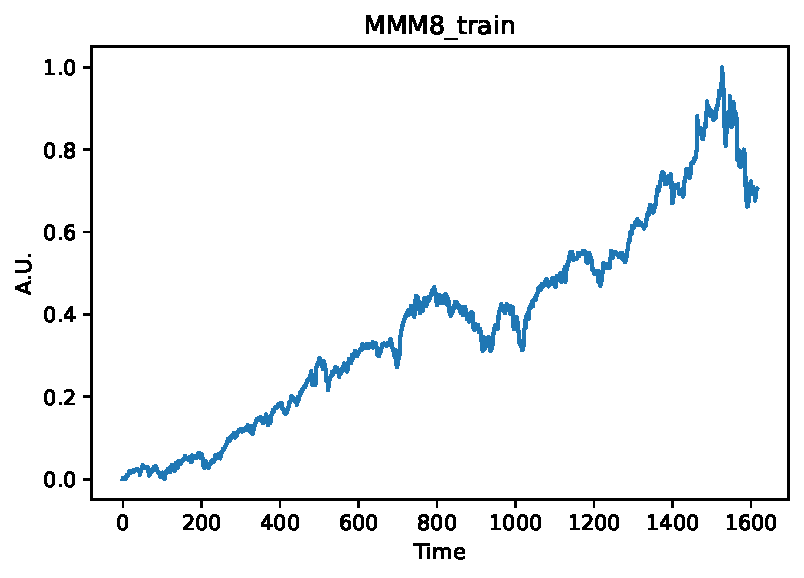
\includegraphics[width=\textwidth]{../img/MMM8_train.pdf}
         \caption{Train set (before COVID-19)}
     \end{subfigure}%
     \begin{subfigure}[b]{0.5\textwidth}
         \centering
         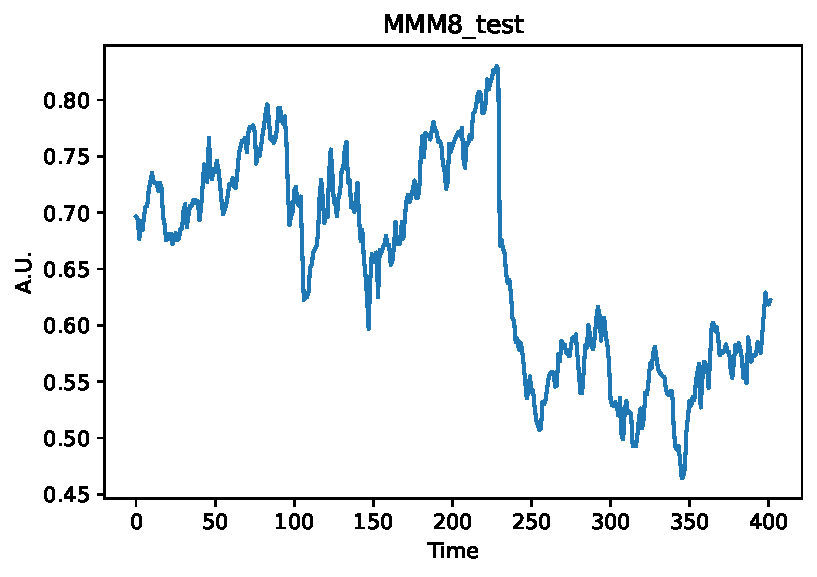
\includegraphics[width=\textwidth]{../img/MMM8_test.pdf}
         \caption{Test set (before COVID-19)}
     \end{subfigure}
     \hfill
     \begin{subfigure}[b]{0.5\textwidth}
         \centering
         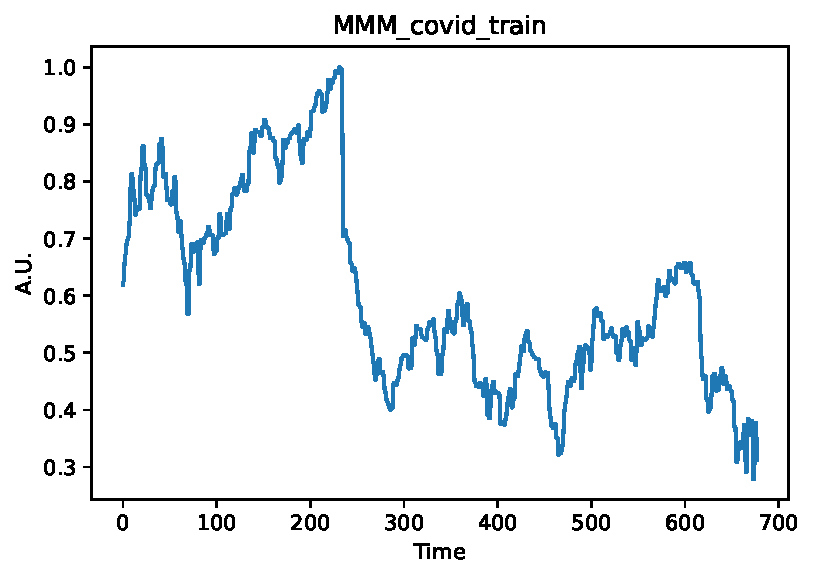
\includegraphics[width=\textwidth]{../img/MMM_covid_train.pdf}
         \caption{Train set during COVID-19}
     \end{subfigure}%
     \begin{subfigure}[b]{0.5\textwidth}
         \centering
         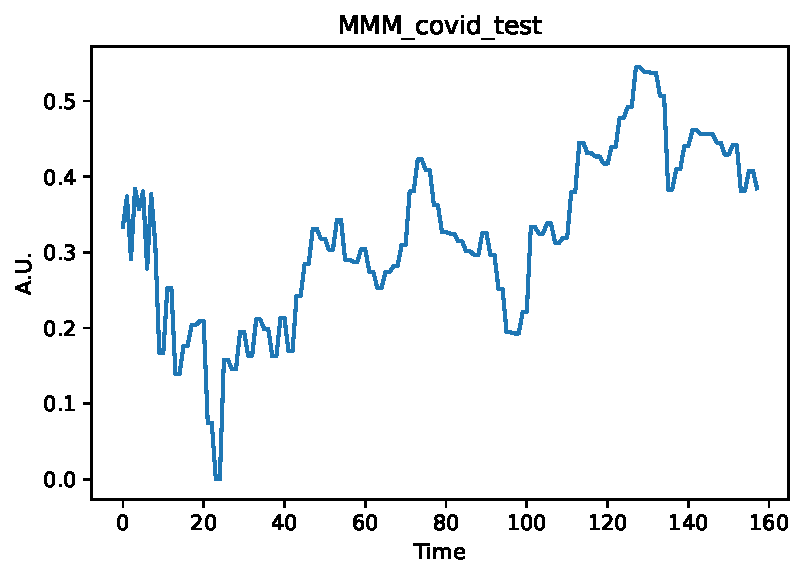
\includegraphics[width=\textwidth]{../img/MMM_covid_test.pdf}
         \caption{Test set during COVID-19}
     \end{subfigure}
    \caption{Stock markets of a company before and during COVID-19 \cite{chandra2021bayesian} (\href{https://github.com/stevengogogo/ECEN649_FinalProject/blob/main/script/EXP_data_visualization.ipynb}{source code}). The training set and testing set is recorded from the different time frame. The objective of \cite{chandra2021bayesian} is to fit each dataset with the same pipeline.}
    \label{fig:data-series}
\end{figure}


The state-space reconstruction is based on Taken's embedding theorem that guarantees the embedding time series (Eq. \ref{eq:window}) retains the manifold of the original dynamics\cite{takens1981detecting}.

\subsection{Framework}

The sequential neural network with one hidden layer is used for the regression problem. The activation function is $\tanh$\footnote{Notebooks and source code is provided at \url{https://github.com/stevengogogo/ECEN649_FinalProject}.}.

The implementation is based on \textit{Haiku} \cite{haiku2020github}, a neural network library with \textit{JAX} backend \cite{jax2018github}.


The input dimension is equal to the window size ($m$, Eq. \ref{eq:window}), and the output dimension corresponds to the prediction horizon ($n$, Eq. \ref{eq:ywindow}). The hidden layer contains 128 nodes. In practice, the properties of the Bayesian neural networks are saved with standard fixed-point neural networks and sampled parameters.


\subsection{Training}

The training process leverages the Bayes theorem (Eq. \ref{eq:bayes}):

\begin{equation}
P(\theta | D) \propto P(D|\theta) P(\theta)
\label{eq:bayes}
\end{equation}

where $\theta$ are parameters and $D$ is dataset. The prior distribution 

\begin{equation}
P(\theta) \sim Normal(0, \Sigma)
\end{equation}


Because there is no closed form of the posterior distribution, a Metropolis-adjusted Langevin algorithm (MALA) is applied to approximate the posterior probability density, and the gradient of probability is calculated via automatic differentiation. The Langevin algorithm provides a better acceptance rate compared to the naive Metropolis-hasting algorithm\cite{roberts1998optimal}. 

The sampling process is divided into three steps:

\begin{enumerate}
    \item \textbf{Initiation} The initiation step uses the prior distribution to sample initial parameters.
    \item \textbf{Proposal} The proposed step uses proposal distribution to generate a  parameter set. This step is optimized by a variety of approaches\cite{jospin2022a}: Hamiltonian Monte Carlo\cite{neal1996, neal2011}, MALA, and other gradient-based methods provide \textit{smart} sampling to yield better mixing and acceptance rate. These approaches are available at \textit{jax-bayes} package\footnote{https://github.com/jamesvuc/jax-bayes}. In MALA, the stochastic differential equation is solved to generate a new state. This approach is inspired by the physical diffusion and has an optimal acceptance rate $0.574$\cite{roberts1998optimal}.
    \item \textbf{Update} The generated sample is decided to accept or reject with the ratio of the probability of current and proposed states. Though the ratio is measured with different methods, the purpose is to avoid integrating the marginal probability of posterior distribution.
\end{enumerate}


The log-likelihood is used to avoid numerical instability when encountering small numbers. In practical (Fig. \ref{fig:training-log}), the log-likelihood can be $10^{-14}$. 

\subsection{Difference from the \cite{chandra2021bayesian}}

In \cite{chandra2021bayesian}, the parallel tempering method is used to train the Bayesian neural network. The source code of \cite{chandra2019langevin} is implemented by NumPy and Multiprocessing. In this project, we are exploring one or several sampling methods and leveraging the just-in-time compilation (JIT) powered by JAX\cite{jax2018github}. The sampling process is compiled to machine code and can be moved to hardware acceleration such as GPU/TPU.


\section{Results}

\subsection{Suboptimal training with MALA}

The iteration of $5\times 10^4$ is used to derive the posterior distribution. Each iteration yields $30$ samples to calculate the log-likelihood. The training log (Fig. \ref{fig:training-log}) shows that more iteration is needed to achieve a higher log-likelihood. 

\begin{figure}[h]
    \centering
    \begin{subfigure}[b]{0.5\textwidth}
        \centering
        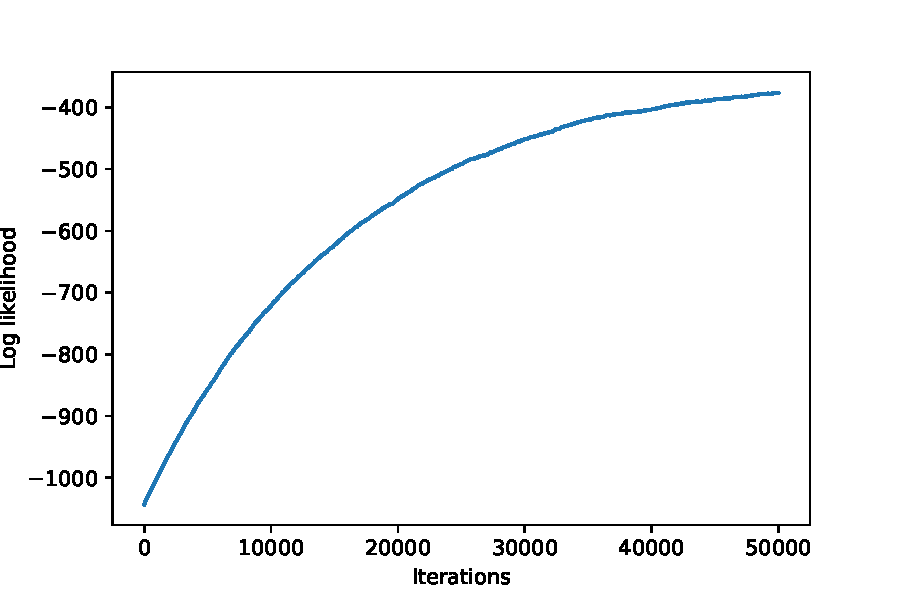
\includegraphics[width=\textwidth]{../img/training_MALA_50000-iter.pdf}
        \caption{Training loss (likelihood).}
        \label{fig:training-log}
    \end{subfigure}%
    \begin{subfigure}[b]{0.5\textwidth}
        \centering
        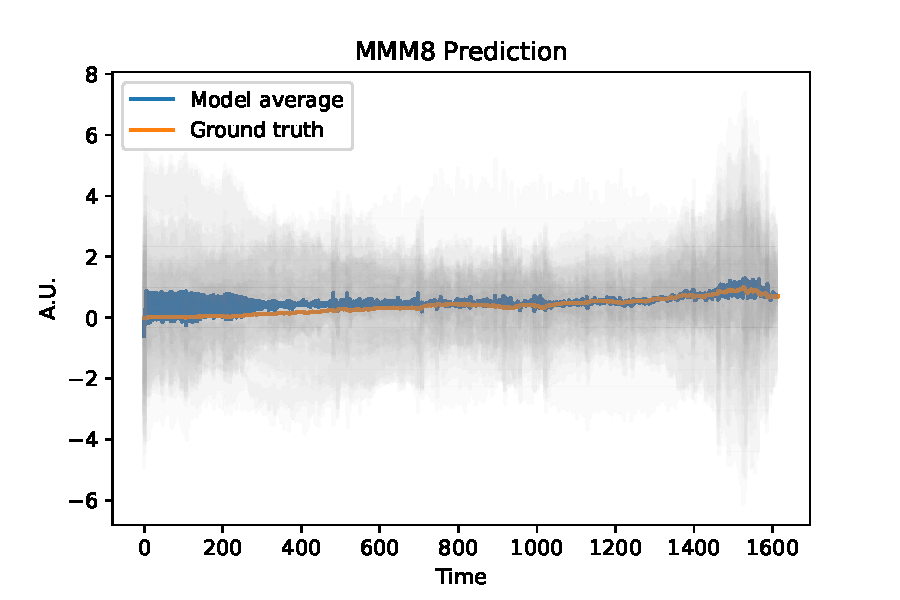
\includegraphics[width=\textwidth]{../img/prediction_MALA_50000-iter.pdf}
        \caption{Prediction (training set)}
        \label{fig:pred-sub}
    \end{subfigure}
    \caption{Training with MALA method. The training process took $30$ min on MacPro M1 Chip. (b) Prediction is made by sampling $30$ times. Each time series is plotted in semi-transparent gray. The mean and ground truth are plotted, respectively. (See \href{https://github.com/stevengogogo/ECEN649_FinalProject/blob/main/script/EXP_fit_time_window.ipynb}{notebook} for implementation details.)}
    \label{fig:pred}
\end{figure}


\bibliography{ref}


\section{Supplemental Materials}

\begin{table}[h]
    \centering
    \begin{tabularx}{\textwidth}{cX}
       \textbf{Resources} & \textbf{Description} \\
       \hline
       \href{https://github.com/sydney-machine-learning/Bayesianneuralnet_stockmarket}{Source code  of \cite{chandra2021bayesian}} & See primary paper\cite{chandra2021bayesian}. This paper applied langevin-gradient parallel tempering from \cite{chandra2019langevin} with stock data under the influences of COVID-19\\\hline
       \href{https://github.com/sydney-machine-learning/parallel-tempering-neural-net}{Source code of \cite{chandra2019langevin}} & See secondary paper\cite{chandra2019langevin} that propose parallel computing of langevin gradient Monte Carlo for Bayesian neural network\\\hline
        \href{https://github.com/sydney-machine-learning/Bayesianneuralnet_stockmarket/blob/master/code/datasets/raw/DAI.DE.csv}{Raw data}  & The original dataset with opened, closed, highest, lowest prices within a day. 1267 days recorded.  \\\hline
       \href{https://github.com/sydney-machine-learning/Bayesianneuralnet_stockmarket/blob/master/code/datasets/600118.SS_1_train.txt}{Processed dataset}  & Filtered dataset. In \cite{chandra2021bayesian}, only one feature is used per day. Noted that the data is non-stationary  \\\hline
       \href{https://github.com/sydney-machine-learning/Bayesianneuralnet_stockmarket/blob/6d24cf25115b6517e3099249bc657674f6b9b98f/code/pt_timeseries_regression.py\#L36-L142}{Bayesian framework} & The implementation is based on \texttt{NumPy}, and the parallel tempering is based on \texttt{multiprocess} package. The computation requires multiprocessing with CPUs.\\
       \href{https://github.com/jamesvuc/jax-bayes}{Jax-Bayes} & Bayesian inference with Jax\cite{jax2018github}.\\\hline
       \href{https://github.com/stevengogogo/ECEN649_FinalProject}{ECEN649\_FinalProject} & Project code and documentation
    \end{tabularx}
    \caption{Resources table.}
    \label{tab:my_label}
\end{table}


\end{document}